\documentclass{llncs}

\usepackage{pbox}
\usepackage[utf8]{inputenc}
\usepackage{url}
%% This was made necessary to break` long URLs, no other system I tried worked and a few URLs still fail; see http://tex.stackexchange.com/a/10419/60582 
\makeatletter
\g@addto@macro{\UrlBreaks}{\UrlOrds}
\makeatother
\usepackage{graphicx}
\graphicspath{{./images/}}

\title{Using hybrid human-machine workflows to create geospatial data}

\author{AUTHOR 1\inst{1}, AUTHOR 2\inst{1} \and AUTHOR 3\inst{2}}
\institute{INSTITUTE 1 \email{EMAIL FOR AUTHOR 1} \and INSTITUTE 2}

\date{December 2015}

\begin{document}

\maketitle

\begin{abstract}
As more open data is published by governments and organisations, the task of creating new data evolves from being a ground-up process - where data is collected and shaped from scratch - to an enhancement process, where pre-existing sources and original additions merge into new, valuable data products. 

Machine learning, computer vision and automation in general can't (yet?) address all challenges in this area, and available data, computation and original contributions by human participants - e.g. through crowdsourcing - need integration and enabling each other through hybrid human-machine workflows. 

In this paper we present a possible application of this model, and setup a platform to deal with a real world use case: the creation of "OLAF", an open dataset of all valid UK addresses, starting from available open geospatial data and augmenting it through computational inference and crowdsourcing. Experimental evaluation show the feasibility and effectiveness of the approach.
\end{abstract}

\begin{keywords}
Crowdsourcing, Geographic Information, hybrid human-machine systems, open data 
\end{keywords}

\begin{itemize}
    \item MAX 18 PAGES
    \item OPEN POINTS
        \begin{itemize}
            \item RESEARCH QUESTION, DESCRIPTION AND ANALYSIS OF THE FINAL EXPERIMENTS ARE STILL MISSING. WHAT CAN BE DONE THAT IS INTERESTING, RELEVANT TO RESEARCH AND FITS THE TIME AVAILABLE?
        \end{itemize}
    \item WEAKNESSES 
        \begin{itemize}
            \item STRONG FOCUS ON USE CASE, POOR GENERALISATION, BUT IS IT NECESSARY?, GIVEN THE CONFERENCE'S EXPLICIT INTEREST IN "Use cases and experiences with human computing and crowdsourcing applications" \url{http://icwe2016.inf.usi.ch/topics#crowd}
            \item ARGUABLE CHOICE OF NOT USING GOLD TESTS
            \item I LIKE THE IDEA OF THE "SOCIAL MACHINE MIX" I PRESENT, BUT THAT SHOULD PROBABLY BE A PAPER OF ITS OWN, UNLESS I CAN FIND SOMEONE WHO DEVELOPED THE SUBJECT BEFORE ME
            \item WON'T HAVE TIME TO DEVELOP ROBUST STATISTICAL DISCUSSION OF THE RESULT, E.G. EXPECTED DISTRIBUTION OF THE WORKER SUBMISSIONS, POSSIBILITY TO USE THAT TO DETECT ANOMALIES ETC., LOTS OF POTENTIAL THERE
            \item I STILL FEEL LIKE I DON'T HAVE A SUFFICIENT AWARENESS OF LITERATURE AROUND ALL SUBJECTS I TOUCH, THERE COULD BE PAST WORK ABOUT ALMOST EVERYTHING I DISCUSS
            \item QUANTITATIVE PROOF OF THE INFERENCE ALGORITHMS BEING EFFECTIVE (WHAT I WANTED FROM CHECKING THE ORDNANCE SURVEY DATA)
        \end{itemize}
\end{itemize}

\section{Introduction}

\subsection{Crowdsourcing}

    Crowdsourcing is {[}...{]}. More generally {[}SOME LIGHTWEIGHT REFERENCE TO WHAT A SOCIAL MACHINE IS{]} [{[}BLAH BLAH SOCIAL MACHINES AS POSSIBLY ONE OF THE ONLY WAYS TO SOLVE PROBLEMS LIKE THIS + SOME EXCUSE TO CITE \cite{OReilly:2015uo}{]}

\subsection{Crowdsourcing Geographic Information}

    Among the many applications of crowdsourcing is the collection and maintenance of geospatial data, or "Geographic Information" (GI).
    
    Although it is commonly recognised for GI to have a significant economic and social value \cite{Sui:2012uf}[THIS IS A REFERENCE TO AN ENTIRE BOOK, LIKELY UNSUITABLE], the effort national mapping and cadastre agencies (NMCAs) worldwide put into producing and updating cartography has been in decline for several decades \cite{ESTES:1994vz}. In the U.S., for example, the Geological Survey (USGS) no longer attempts to update its maps on a regular basis and the National Research Council promotes a vision in which {[}...{]} \cite{Committee:1993vp}.
    
    {[}Somewhere in the literature someone said that the emergence of VGI was actually suggested by one of those authorities{]}
    
    Crowdsourcing GI is then seen as the cost effective and "good enough" solution to this problem [CITATION OF SOME SCHOLAR SAYING THAT GOOD ENOUGH IS... GOOD ENOUGH]. The phenomenon of {\it Volunteered} Geographic Information (VGI) in particular was studied extensively since the term was coined \cite{Goodchild:2007vt}. Developing understanding of VGI was made possible by the success of services such as Wikimapia\footnote{\url{http://wikimapia.org/}.} or OpenStreetMap\footnote{\url{http://www.openstreetmap.org/}.}. The latter is likely the best known VGI-based mapping service available today.

\subsection{Open data and open Geographic Information}

    Open data is data that anyone can access, use and share\footnote{\url{http://theodi.org/faq}.}. 
    
    NMCAs, as governments and private organisations, are becoming more sensitive to the opportunities arising from publishing and re-using open data. In Great Britain, for example, since 2015 the local NMCA Ordnance Survey\footnote{\url{http://www.ordnancesurvey.co.uk/}.} has released in the open a substantial volume of data that was previously available to the public as commercial products only, e.g. "Open Names"\footnote{\url{https://www.ordnancesurvey.co.uk/business-and-government/products/os-open-names.html}.}, a place-name index, and "Open Roads"\footnote{\url{https://www.ordnancesurvey.co.uk/business-and-government/products/os-open-roads.html}.}, the generalised geometry and network connectivity of the road network.
    
    The availability of such high quality and authoritative sources becomes a substantial enabler for the creation of new, original geospatial data. There where GI could only be created from scratch - as in OpenStreetMap's case when it was started in the UK in 2007 - it is now possible to rather focus the effort of the crowd on complementing what is already available, or augmenting it.

\subsection{Crowdsourcing open data}

    The work described in this paper took place in the context of a larger research programme aimed at assessing the feasibility of building original open data by using non-expert human contributions, technology systems and, where available, other pre-existing open data. 
    
    Although most of the effort of producing and releasing open data is commonly expected of governments and businesses, there are industry sectors and domains of knowledge where resistance to change can halt or substantially slow down this process. Demand and offer for open data is strongly suppressed, for example, due to failure in recognising open data-enabled business models, restrictive legislative and patent systems, or charging for public datasets \cite{shadboltpaf}. 
    
    The assumption at the base of our research is that the people's contribution is necessary to address this problem. People can be enabled, through technology, to capture and curate data, alongside what is already published by governments and businesses. Crowdsourcing is just one of the formulae by which socio-technical systems can be built for this purpose. This contribution is instrumental to delivering and curating the open data needed to build and operate a comprehensive {\it national information infrastructure} (NII).

\subsection{Challenges of crowdsourcing geospatial data}

    Two groups of challenges are relevant to the availability of good quality geospatial open data: on one side, exploiting it to improve the quality and enhance the functionality of pre-existing VGI initiatives, and, on the other, unleash completely new products and services.
    
    [CHALLENGE OF MAINTENANCE, AFTER COLLECTION]
    
    [SHOULD I WRITE MORE ABOUT THE OTHER CHALLENGES, TOO?]
    
    Completeness is a key element in the quality of geospatial data. In this paper we propose a method to improve the coverage of existing geospatial data where - for any reason - it is not possible to get volunteers to survey one specific geographical area or provide more detail than what is available already. This was described, for example, by **** , observing how OpenStreetMap volunteers naturally tend to avoid ***.
    
    {[}
    Add
    \begin{itemize}
    	\item {[}rationale of why we thought this was relevant, some justification in literature review{]}
    	\item {[}novelty of what we propose{]}
    \end{itemize}
    {]}
    
    {(}...{)}

\subsection{The Open Legal Address File}

    The main use case for this research is the attempt of creating a new geospatial dataset that is functionally equivalent to the "Postcode Address File" or "PAF"\footnote{PAF is a registered trademark by Royal Mail plc. For convenience we won't show the registered trademark sign "\textregistered" in this document every time we refer to it.}: a commercial dataset listing all known valid addresses and postcodes for the UK at a given point in time. 
    An act of law\footnote{The Postal Service Act 2000, part VII, article 116 \cite{postalserviceact2000}.} makes PAF ownership of the Royal Mail: the ex-postal service monopolist in the UK, now a public limited company with only a 30\% of shares controlled by the Government\footnote{The Postal Services Act 2011 plans to reduce the Government control down to 10\% \cite{postalserviceact2011}.}. The same act of law requires Royal Mail to make PAF available on "reasonable terms" to "any person who wishes to use it".
    
    To this day, though, the "reasonable terms" translated only into PAF being made available by Royal Mail and its resellers as a commercial product\footnote{As an end user who wants to access PAF's data one may incur Royal Mail licence fees going from \pounds0.012 per transaction on a public website to \pounds90,000 per year for unlimited internal use by a corporate group. Even charitable organisation may not take advantage of free PAF access unless their income is less than \pounds10m/year.}. This is considered an anomaly by many, as "reasonable terms for the external use of PAF data by third parties should be no more than the marginal cost of distribution (...)" \cite{odugresponse}. 

    To further limit the opportunities for PAF to be made open, in October 2013 Royal Mail and its assets were privatised, including PAF\footnote{\url{http://www.theguardian.com/uk-news/2014/mar/17/royal-mail-privatisation-ministers-rebuked-selling-data}}. The UK Parliament House of Commons' Public Administration Select Committee, just a few month later, called this "unacceptable and unnecessary" and recognised that PAF's "disposal for a short-term gain will impede economic innovation and growth" \cite{pascod}.

    This makes the opportunity of creating an alternative to PAF an ideal case study. We will call this the "Open Legal Address File", or "OLAF". The term "legal addresses" refers to all addresses that are, by law, in the public domain, hence have no restrictions in terms of intellectual property or privacy protection and can be published as open data\footnote{Legal addresses belong to either or both of the following two categories: a) they are the addresses of current or past UK residents who are or were registered on the public electoral register, and b) they are the addresses of past or present UK companies that are or were registered at the relevant British registrar, such as Companies House for England and Wales.}.

    {[}Definition of address{]}
    
    Many complementary and/or alternative strategies are possible and need to be used jointly to build OLAF. Among these is the opportunity to re-use published open datasets of addresses so to infer the existence of more addresses. 
    
    E.g. it is intuitive that if some source refers to the existence of house numbers 3, 5 and 9 in some street, and all are associated to the same postcode, it is very likely that number 7 exists as well and is associated to the same postcode\footnote{House numbering and postcode association are heavily dependant of the conventions used in the country the problem is applied to. This paper always refers to the UK conventions.}. It is shown experimentally that the method is effective, as it can produce large volumes of addresses from available open data\footnote{This was tested against the single largest known source of addresses open data for England and Wales: Land Registry's "Price Paid Data". See \url{https://www.gov.uk/government/collections/price-paid-data}.}.
    
    The experiments described in this paper implement the above strategy only, and  use crowdsourcing to validate sets of inferred addresses, as participants are asked to virtually survey the streets using pictures sourced from Google Street View.
    
    It has to be noted that not all existing house numbers are visible by surveying a street. E.g. there are no obligations in the UK to affix a house number or house name sign. Moreover, some of the house numbers may be associated to dwellings that are not visible unless the property is accessed, beyond what Google Street View's photos can capture.
    
    {(}...{)}
\section{Background}

\subsection{The Open Legal Address File}

    The main use case for this research is the attempt of creating a new geospatial dataset that is functionally equivalent to the "Postcode Address File" or "PAF"\footnote{PAF is a registered trademark by Royal Mail plc. For convenience we won't show the registered trademark sign "\textregistered" in this document every time we refer to it.}: a commercial dataset listing all known valid addresses and postcodes for the UK at a given point in time. 
    An act of law\footnote{The Postal Service Act 2000, part VII, article 116 \cite{postalserviceact2000}.} makes PAF ownership of the Royal Mail: the ex-postal service monopolist in the UK, now a public limited company with only a 30\% of shares controlled by the Government\footnote{The Postal Services Act 2011 plans to reduce the Government control down to 10\% \cite{postalserviceact2011}.}. The same act of law requires Royal Mail to make PAF available on "reasonable terms" to "any person who wishes to use it".
    
    To this day, though, the "reasonable terms" translated only into PAF being made available by Royal Mail and its resellers as a commercial product\footnote{As an end user who wants to access PAF's data one may incur Royal Mail licence fees going from \pounds0.012 per transaction on a public website to \pounds90,000 per year for unlimited internal use by a corporate group. Even charitable organisation may not take advantage of free PAF access unless their income is less than \pounds10m/year.}. This is considered an anomaly by many, as "reasonable terms for the external use of PAF data by third parties should be no more than the marginal cost of distribution (...)" \cite{odugresponse}. 

    To further limit the opportunities for PAF to be made open, in October 2013 Royal Mail and its assets were privatised, including PAF\footnote{\url{http://www.theguardian.com/uk-news/2014/mar/17/royal-mail-privatisation-ministers-rebuked-selling-data}}. The UK Parliament House of Commons' Public Administration Select Committee, just a few month later, called this "unacceptable and unnecessary" and recognised that PAF's "disposal for a short-term gain will impede economic innovation and growth" \cite{pascod}.

    This makes the opportunity of creating an alternative to PAF an ideal case study. We will call this the "Open Legal Address File", or "OLAF". The term "legal addresses" refers to all addresses that are, by law, in the public domain, hence have no restrictions in terms of intellectual property or privacy protection and can be published as open data\footnote{Legal addresses belong to either or both of the following two categories: a) they are the addresses of current or past UK residents who are or were registered on the public electoral register, and b) they are the addresses of past or present UK companies that are or were registered at the relevant British registrar, such as Companies House for England and Wales.}.

    {[}Definition of address{]}
    
    Many complementary and/or alternative strategies are possible and need to be used jointly to build OLAF. Among these is the opportunity to re-use published open datasets of addresses so to infer the existence of more addresses. 
    
    E.g. it is intuitive that if some source refers to the existence of house numbers 3, 5 and 9 in some street, and all are associated to the same postcode, it is very likely that number 7 exists as well and is associated to the same postcode\footnote{House numbering and postcode association are heavily dependant of the conventions used in the country the problem is applied to. This paper always refers to the UK conventions.}. It is shown experimentally that the method is effective, as it can produce large volumes of addresses from available open data\footnote{This was tested against the single largest known source of addresses open data for England and Wales: Land Registry's "Price Paid Data". See \url{https://www.gov.uk/government/collections/price-paid-data}.}.
    
    The experiments described in this paper implement the above strategy only, and  use crowdsourcing to validate sets of inferred addresses, as participants are asked to virtually survey the streets using pictures sourced from Google Street View.
    
    It has to be noted that not all existing house numbers are visible by surveying a street. E.g. there are no obligations in the UK to affix a house number or house name sign. Moreover, some of the house numbers may be associated to dwellings that are not visible unless the property is accessed, beyond what Google Street View's photos can capture.
    
    {(}...{)}
\section{Approach}

\cite{Difallah:2012ty}

[MAKE POINT ABOUT ONE OF THE ORIGINAL INTUITION POINTS BEING REDUCING THE ORIGINAL PROBLEM TO AN IMAGE LABELLING PROBLEM, IT'S NOT NECESSARILY OBVIOUS]
[USE \cite{Quinn:2011dj} FOR THE DEFINITION OF THE AGGREGATION PROBLEM]
[HIGHLIGHT HOW, DIFFERENTLY THAN MOST OF CROWDSOURCING IMAGE LABELLING USE CASES, HERE WE'RE COLLECTING TWO LABELS PER "SUBJECT", AND THEY'RE PRACTICALLY INDEPENDENT]
[HIGHLIGHT HOW THE SET OF POSSIBLE VALUES FOR THE LABELS IS NOT LIMITED, IT'S MORE LIKE AN NxN SPACE, N BEING THE SET OF NATURAL NUMBERS, WHERE THE FIRST N REPRESENTS THE ACTUAL NUMBERS 1, 2, 3... AND THE SECOND N THE LETTERS IN THE POSTFIX 1 -> A, 2 -> B, ..., 27 -> AA ...]

\subsection{The social machine mix}

    Although the OLAF data is conceptually simple, assembling such a large dataset as OLAF while assuring sufficient quality still is a complex task.
    
    It is our hypothesis that, to make the best use of pre-existing open data and potentially available technology and human resources, such a problem must be decomposed in a series of complementary sub-problems, each developing parts of its scope and leveraging the peculiarity of its specifications. Each problem, then, can be solved by designing a dedicated socio-technical system, or social machine. This decomposition can take place over several iterations, hence creating a hierarchy of systems that we will call the "social machine mix". 
    
    [THERE SHOULD BE AN IMAGE HERE BUT IMAGE POSITIONING IN LATEX IS TRICKY]

    \begin{figure*}
    	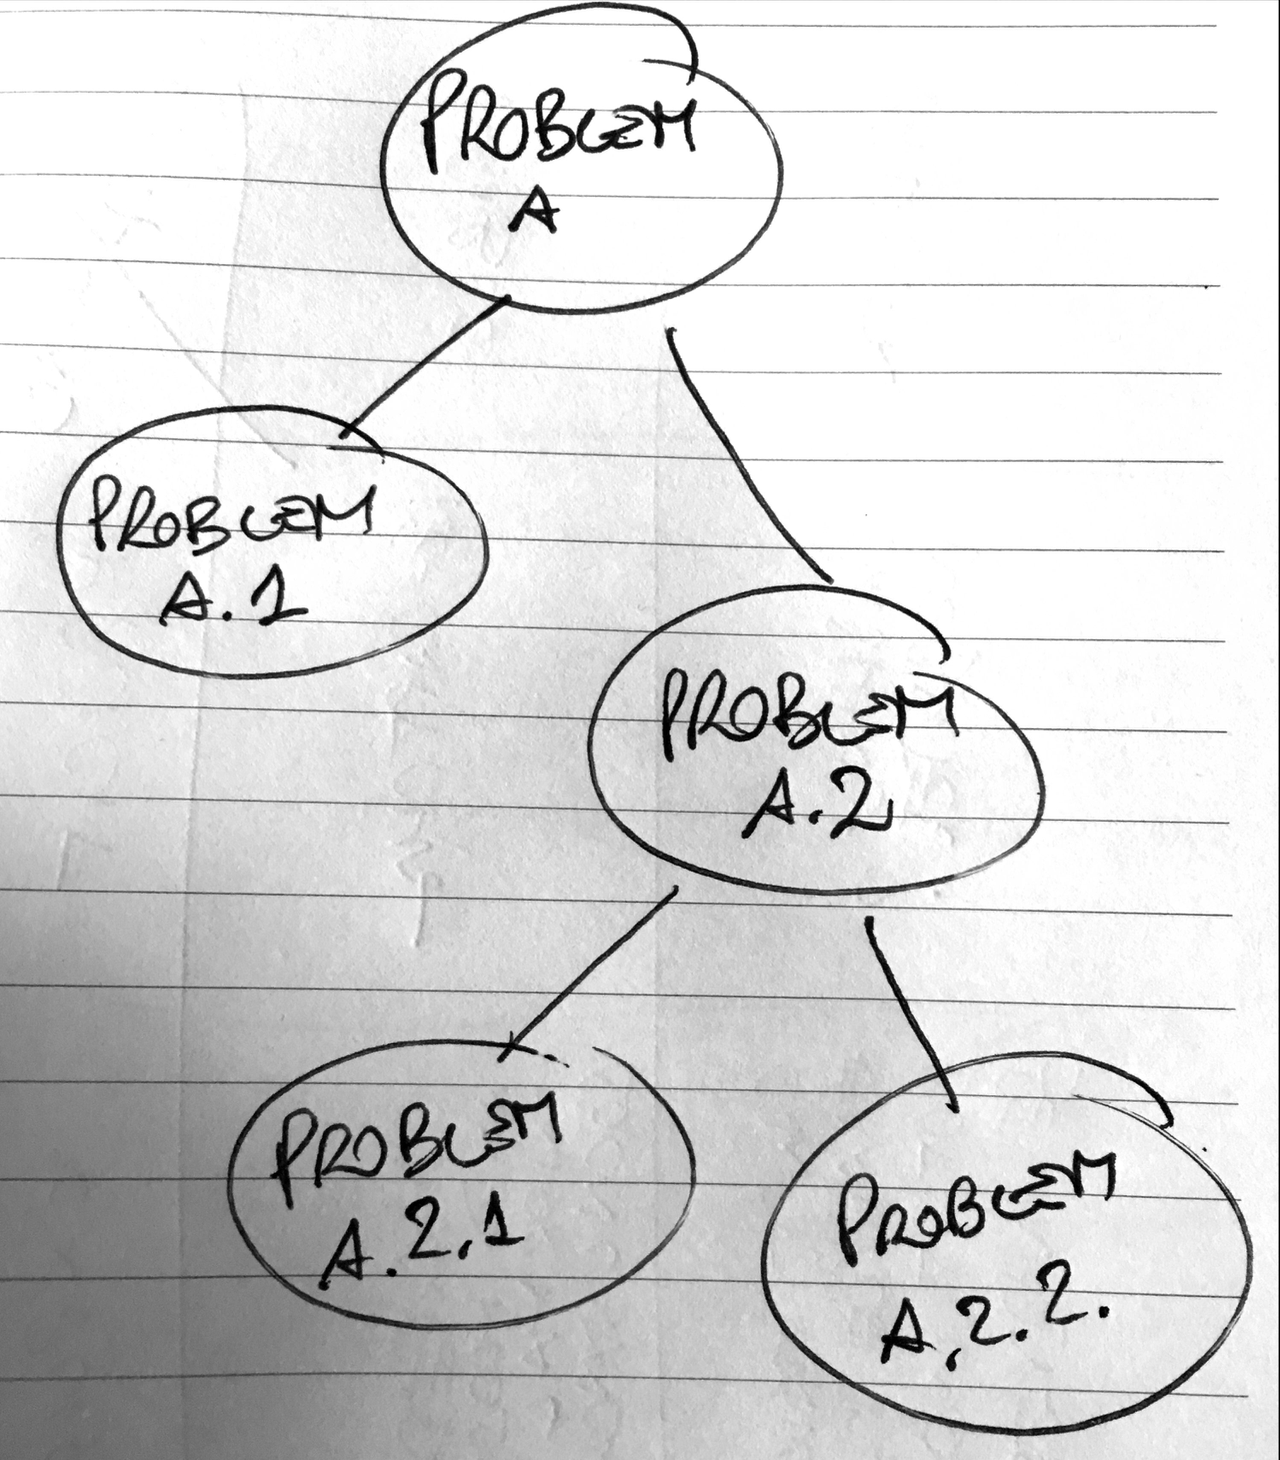
\includegraphics[width=0.95\textwidth]{social-machine-mix-1.png}
    	\caption{This picture should not be here, but apparently it is a nightmare in LaTeX.}
    	\label{fig:social_machine_mix_1}
    \end{figure*}
    
    \textbf{The central role of pre-existing open data.} 
    
    [THIS IS AN INTERESTING STATEMENT, I WONDER IF IT CAN BE GENERALISED] The main driver determining the possible decompositions of the original problem into a hierarchy of sub-problems is the availability of pre-existing and reliable open data. There are two reasons for that.

    \begin{itemize}

        \item The first and more intuitive reason is an assumption: no social machine can produce data in a more effective way than re-using a pre-published, reliable dataset is.  
        
        Hence, re-using existing open data will always be prioritised in respect to re-creating the same, e.g. using crowdsourcing. The focus of social machines in the overall mix should rather be on: a) on creating original data where the same cannot be sourced or computed, and b) on leveraging those skills where humans outperform machines. 
        
        The obvious example of this is using human contributors to survey the streets, being this in person in the physical world, or by examining pictures of the locations, that is how crowdsourcing is used in the system described later in this paper.

        \item The second reason is that open data can be instrumental to operate a social machine. Even when a dataset is not re-used directly to creating the target output data, it can be used for other functions, e.g. supporting the process by which humans contribute. There will be a clear example of this later in this paper. 

    \end{itemize}

\subsection{Scope restrictions}
    
    [DOES NOT SOUND LIKE IN THE RIGHT PLACE, BUT THE SECTIONS THAT COME AFTERWARDS NEED THIS CLARIFICATION BEFORE] 
    
    To make the problem suitable to research it was simplified as described below. 
    
    \textbf{Open data availability.} Although the overarching objective for OLAF is to achieve UK coverage, the availability of open data differs substantially from one UK country to another. Our approach was based on what is available for England and Wales only, as the two have the richer and most homogeneous open data offering, and their territory is estimated to include the 84\% of the 35m addresses in the UK\footnote{[FOOTNOTE EXPLAINING THE ESTIMATE, LIKELY TO BE MADE USING NO. OF HOUSEHOLDS BY COUNTRY FROM ONS AS AN INDICATION OF NO. OF BUILDINGS HENCE ADDRESSES]}.
    
    The validity of the approach is independent of the geographical region that is the subject of the study, as long is the problem is consistent, e.g. the definition of the address is the same. The moment the same open data used for England and Wales becomes available for Scotland and Northern Ireland, the method can be deployed to produce an UK-wide OLAF without modification. Alternatively, if that would not happen, complementary social machines would need being added to the mix.
    
    \textbf{Sample territory.} Within the territory described above, the experiments were performed to address just a sample of the London area, made of five tiles [MORE TECH DESCRIPTION OF WHAT THEY ARE]. This is the same sample that was used in literature in the past to analyse the performance of other geospatial data crowdsourcing initiatives, e.g. OpenStreetMap in [REFERENCE].
    
    \begin{figure*}
    	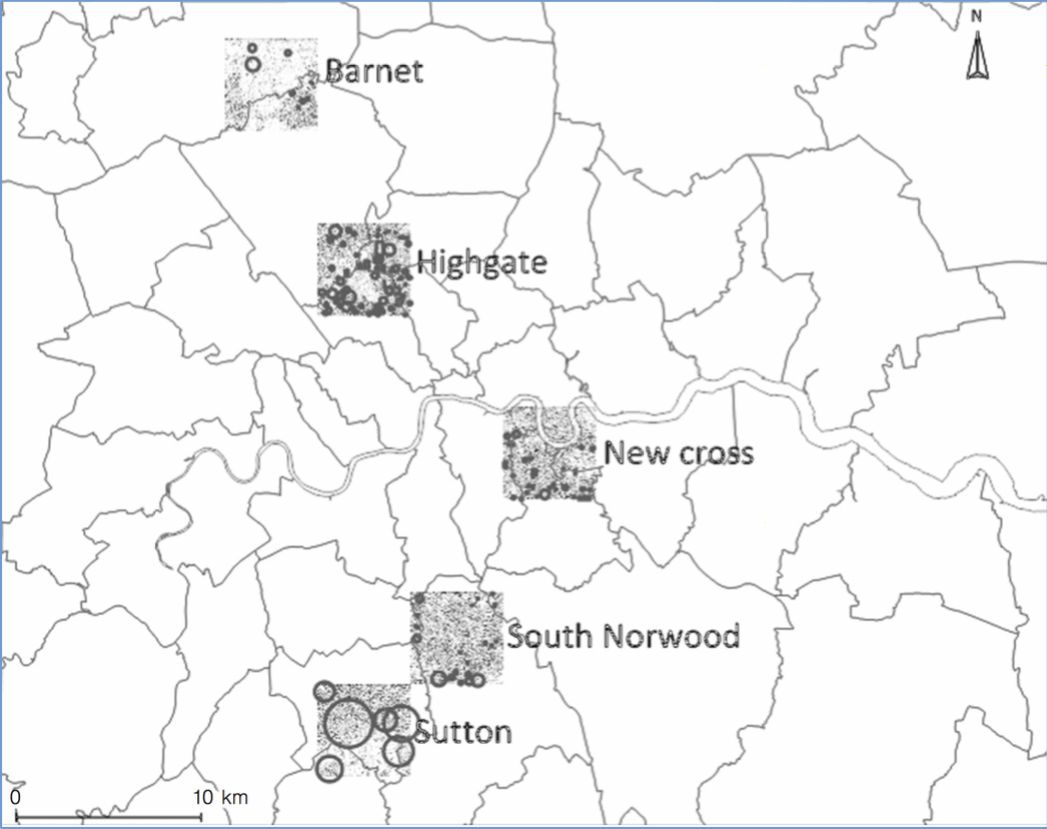
\includegraphics[width=0.95\textwidth]{london-sample-1.png}
    	\caption{This picture should not be here, but apparently it is a nightmare in LaTeX.}
    	\label{fig:london_sample_1}
    \end{figure*}
    
    More precisely, a road is considered in scope if its bounding box, as defined by Ordnance Survey's "Open Names", is completely included in any of the five tiles. 
    
    [SOME WORDING FROM THAT PAPER TO STATE HOW WE DID NOT SIMPLIFY THE PROBLEM BY DOING THIS BUT JUST REDUCED IT IN SIZE].
     
    \textbf{Named vs numbered roads.} Roads that are identified by a number only, e.g. as for motorways, will be considered out of scope.
    
    \textbf{Reliability of the sources.} Only open data from authoritative sources was considered as an option in defining the approach, such as government bodies', and it is assumed to be of the highest possible quality, equivalent to what could be called {\it ground truth}. This allowed the approach not to include any validation of the sources.

\subsection{A social machines mix for OLAF}

    The open data available during our research makes it possible to divide the creation of OLAF in two main sub-problems {\it p1} and {\it p2}. 
    
    \begin{itemize}
        \item {\it p1}: Create a list of all existing {\it house numbers} for each road listed in Ordnance Survey's "Open Names".
        \item {\it p2}: Create a list of all existing {\it house names} for each road listed in Ordnance Survey's "Open Names".
        \item {\it p3}: Create a list of the associations between each of the house number and names above and the list of current\footnote{Postcodes can change. The problem of documenting how addresses change postcode in time is relevant but outside of the scope of research.} postcodes listed in Ordnance Survey's "Open Names". 
    \end{itemize}

    For simplicity, we use the terms "place", "road" and "street" interchangeably, as they are equivalent from a data model perspective in OLAF.

    Open Names "lists definitive place names, roads numbers and postcodes in Great Britain"\footnote{See \url{https://www.ordnancesurvey.co.uk/business-and-government/products/os-open-names.html}.}. It was central to the research work as it is dataset that is functionally closer to the target. OLAF is - in practical terms - equivalent to adding just one dimension to Open Names, that is the list of house names and number for each of its roads. 
    
    Problems {\it p2}\footnote{Note that 98\% of UK addresses are characterised by a house number rather than a house name, so solving {\it p1} is substantially more relevant to achieve completeness in OLAF than {\it p2}.} and {\it p3} are not discussed in this paper. 
    
    Problem {\it p1} can be further decomposed, thanks to the availability of additional open data sources:
    
    \begin{itemize}
        \item {\it p1.1}: Collect the list of house numbers and house names for each existing road as they are referenced in pre-existing open data.
        \item {\it p1.2}: Infer the existence of house numbers from the house numbers collected by {\it p1.1}.
        \item {\it p1.3}: Enable the application of {\it p1.2} by creating the minimum necessary data to trigger more inference.
        \item {\it p1.4}: Correct the output of {\it p1.2}.
    \end{itemize}

    \subsubsection{{\it p1.1}: Collect the list of house numbers and house names for each existing road as they are referenced in pre-existing open data.} 

        References to existing house names and numbers can be found in a few open data publications in the UK. The largest in size is the "Price Paid Data" by the Land Registry (LRPP in the following): a non-ministerial Government department with the responsibility to register the ownership of land and property in England and Wales. Data for each ownership transfer since 1995 - and the full address of the building - is available as open data and updated monthly.
        
        20 years of record make an impressive collection of house names and numbers [MORE ABOUT WHAT THE OUTPUT OF THIS IS]

    \subsubsection{{\it p1.2}: Infer the existence of house numbers from the house numbers collected by {\it p1.1}.} 

        Each culture developed in time a convention for the assignment of house number and names to buildings. In the UK numbering was likely introduced in the early 18th Century as an alternative to house names. Buildings typically are numbered sequentially starting from 1, corresponding to the extremity of the road that is closest to the centre of the town the street is associated to. Odd numbers are on the left-hand side as seen from the centre, even number on the right-hand side. Intermediate properties usually have a number suffixed by one or more letters, this is typical of larger buildings that at some point in time got divided into more smaller dwellings. Modern buildings that have been named by their owner usually retain also a number, that was used by the local government authority during planning.
        
        Centuries of house development and using this system informally of course created many exceptions: e.g. there are buildings for whose house number is zero, places where numbers were assigned consecutively, and house numbers that are simply missing. Simple algorithms, though, have a very high probability to apply the numbering model described above to infer the existence of house numbers from other known house numbers. This is intuitive, as: 
        \begin{itemize}
            \item If we know that one even and one odd house numbers exist in a street, it is likely that all other numbers included within those numbers exist, too (e.g. we can infer 11 and 12 from the existence of 10 and 13)
            \item If we know that two even or odd house numbers exist in a street, it is likely that all other even or odd house numbers included within those numbers exist, too (e.g. we can infer 7 from the existence of 5 and 9, but not 6 and 8, as the right-hand side of the street may not have buildings)
            \item If we know that the same house number in a street is suffixed by two different letters, it is likely that all other letters included within those letters exist, too (e.g. we can infer 14B from the existence of 14A and 14C).
        \end{itemize}
        
        This simple inference is one of the simplest that can be implemented. Other available open data sources enable more complex algorithms, e.g. Ordnance Survey's "Open Maps - Local" [NEED TO CHECK] includes summary shapes for the buildings in each British street, hence enabling the detection of how many buildings are present and suggest how some house numbers may be missing.
        
        {\bf Error in inference.} The described inference criteria add error to the data, made of three components: (i) inferred house numbers that are in reality house names (2) inferred house numbers that in reality exist only in prefixed form instead (e.g. 7A instead of 7), and (iii) addresses that simply do not exist, e.g. because a building was demolished.
        
        We can estimate (i) and (ii) by observing in LRPP. The frequency of addresses identified by a house names instead than a house number is 2\% of the total for the geographic area in scope. This is like saying that 1 out of 50 inferred house numbers was supposed to be a house number instead. The volume of house numbers that exist in prefixed form only instead is [TO CALCULATE, LIKELY INCREDIBLY LOW]. We believe this is an acceptable burden to put on the {\it p1.4} system. 
        
    \subsubsection{{\it p1.3}: Enable the application of {\it p1.2} by creating the minimum necessary data to trigger more inference.} 

        It is clear from the description of problem {\it p1.2} that the inference of house numbers is enabled by the availability of two or more couples of house numbers that act as "seeds" and allow the inference rules to trigger one or more times, for each road.
        
        82\% of the streets in scope are referenced in Land Registry's "Price Paid. The house numbers sourced from {\it p1.1} create opportunities for inference for the 74\% of roads, inferring ~113k house numbers from ~111k known house numbers [DO I NEED TO DESCRIBE THE CALCULATIONS SOMEWHERE IN THE PAPER OR I JUST LINK TO THE GITHUB REPOSITORY WITH THE CODE? THE CODE AT THE MOMENT DOES NOT CALCULATE THE STATISTICS BUT JUST RUNS THE INFERENCE, THIS STUFF WAS CALCULATED 'BY HAND'.]. A substantial number of roads are not described by sufficient data to trigger any inference. 
        
        Because of the above, it suitable to decompose problem {\it p1.3} into two more specialised problems:
        
        \begin{itemize}
            \item {\it p1.3.1}: Enable the application of {\it p1.2} to streets that are not described by pre-existing data.
            \item {\it p1.3.2}: Extend the application of {\it p1.2} beyond the house numbers that are known thanks to pre-existing data.
        \end{itemize}
        
        Problem {\it p1.3.2} is not discussed in this paper. Problem {\it 1.3.1} is about creating the minimum set of data capable of creating the largest sets of inferred house numbers for roads we know nothing of. This means identifying the lowest and highest house numbers for each road for which no house numbers are known\footnote{For simplicity, we did not consider the case where one house number only is known for a street. Those roads are considered as roads with no house numbers.}.

        \begin{figure*}
        	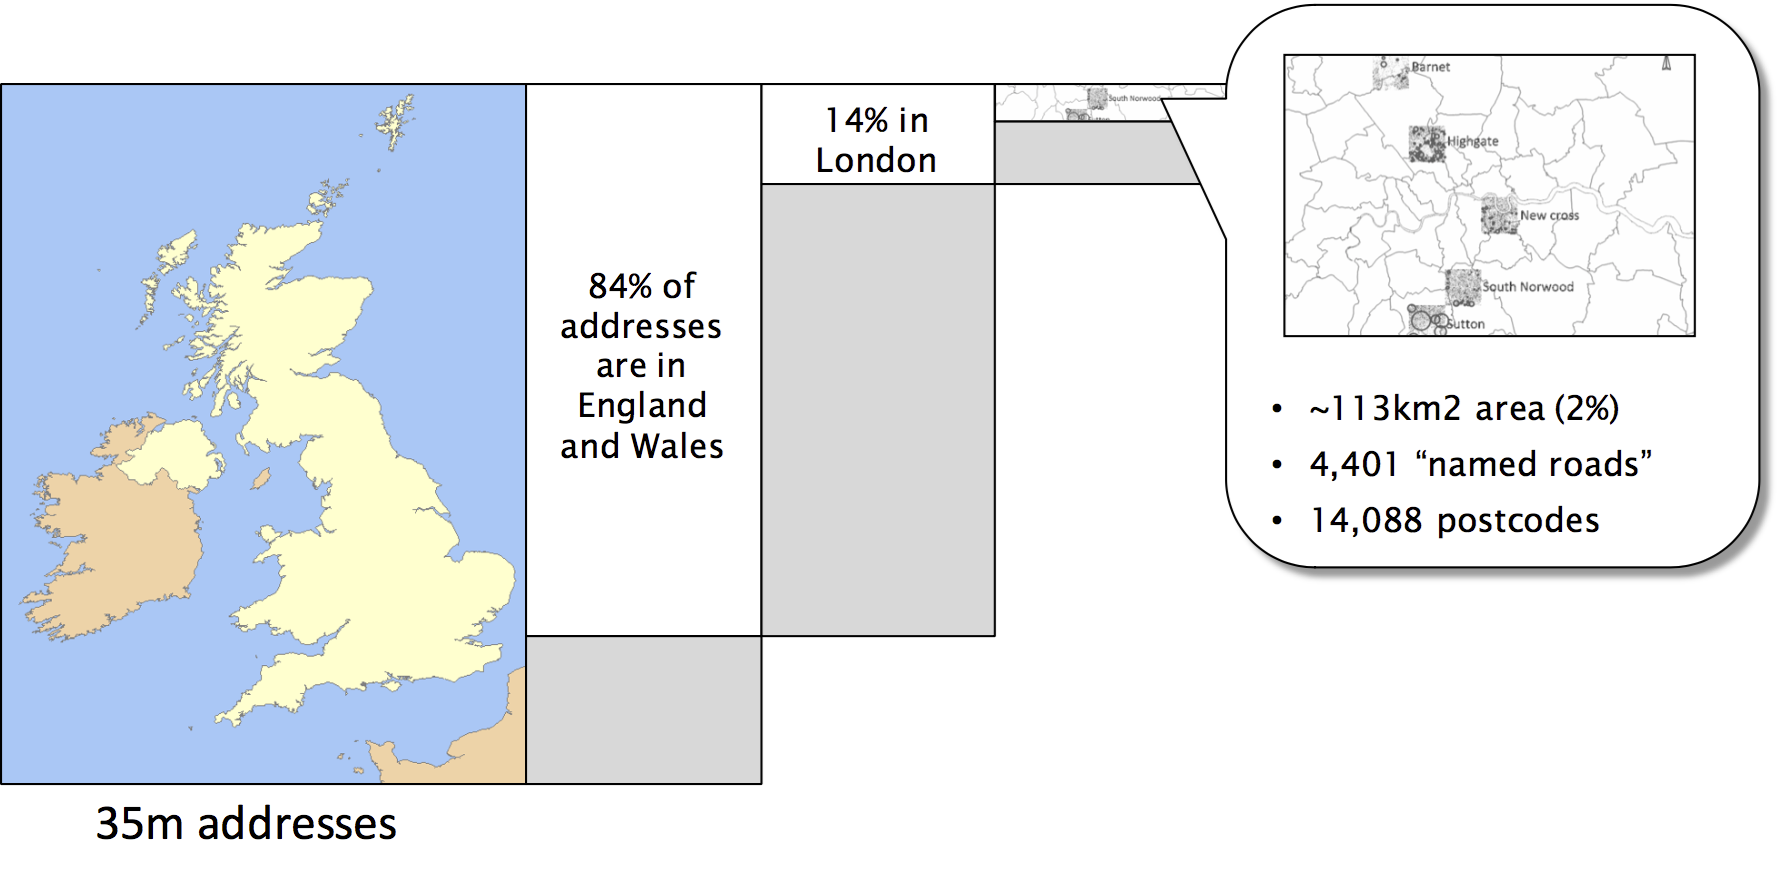
\includegraphics[width=0.95\textwidth]{social-machine-mix-3.png}
        	\caption{This picture should not be here, but apparently it is a nightmare in LaTeX.}
        	\label{fig:social_machine_mix_3}
        \end{figure*}
        
        \begin{figure*}
        	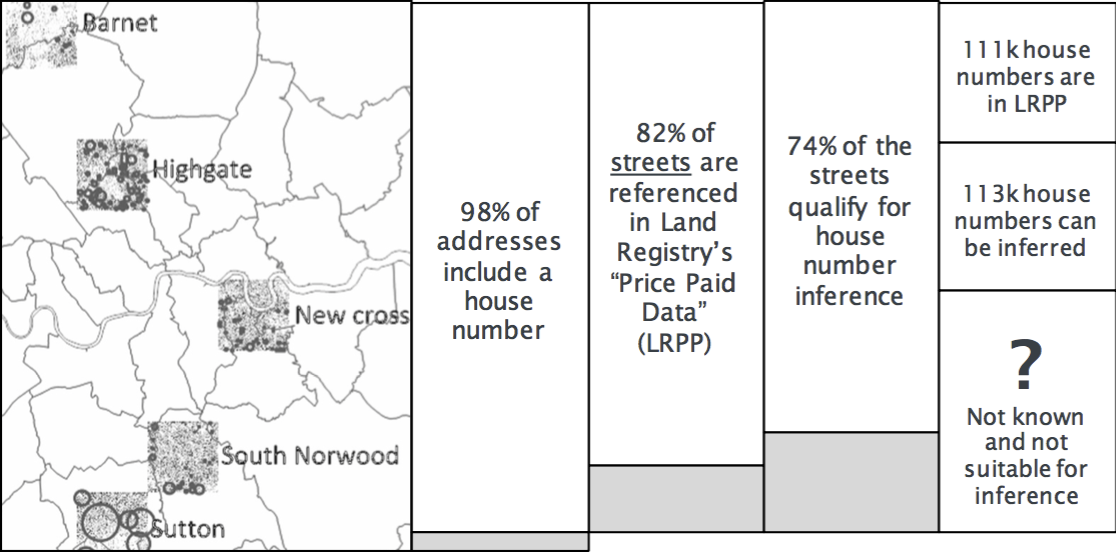
\includegraphics[width=0.95\textwidth]{social-machine-mix-2.png}
        	\caption{This picture should not be here, but apparently it is a nightmare in LaTeX.}
        	\label{fig:social_machine_mix_2}
        \end{figure*}
        
        As no pre-existing open data is available by definition to address this problem, the needed data needs being generated through surveying. 

    \subsubsection{{\it p1.4}: Correct the output of {\it p1.2} through surveying.} 

        Finally, problem {\it p1.4} is about correcting error in {\it p1.2}, typically identifying house numbers that were inferred but do not exist, or that are replaced by house names.
        
        As no pre-existing open data is available by definition to address this problem, the identification of error and the data needed for correction needs being obtained through surveying. 

        Problem {\it p1.4} is not discussed in this paper.

\subsection{Crowdsourcing house numbers to enable inference}

    The focus of the research described in this paper is the solution of problem {\it p1.3.1}. This is not conceptually different than an annotation problem where for each annotated instance there is a single right answer, with a few key differences:
    
    \begin{itemize}
        
        \item For each item subject to annotation, two independent annotations are collected: the lowest and highest visible house numbers. 
        
        There is no use in splitting the task in two, asking one Worker to look for the lowest house number and another to look for the highest. By exploring the pictures of the assigned street the Worker will naturally focus her research on the extremities of the road, where the relevant house numbers are, without knowing in advance which of the two she is finding.
        
        One could argue that the two annotations are not truly independent, as the lowest house number is, by definition, lower than the highest house number. In practical terms, though, the task of surveying a street cannot leverage such mathematical relation. For example, knowing the highest house number won't help the Worker finding the lowest house number, as her finding is rather due toto the observation of the morphology of the street and the progression of nearby house numbers. 
        
        \item The information subject to the annotation could be identified as existing, but the annotation may not be possible anyway. E.g. a Worker will be able to see which the first house in a street is from observing the house numbers on nearby buildings, but vegetation may hide the number. There is also the possibility that Google Street View coverage does not include the surveyed street.
        
        Moreover, unlike other countries, in the UK local authorities do not provide house number plates to the building owners, so this remains their responsibility. Building owners have the option not to affix any plate at all. 
        
        \item There may be nothing to annotate. Because of the nature of the problem, the streets we are using crowdsourcing to collect data about are the ones that appeared little or not at all in pre-existing data, e.g. in Land Registry's Price Paid data over the last 20 years. There likely is a reason for that, e.g. the street may be rural and have few buildings. 
        
    \end{itemize}
    
    The following is a description of the approach that was used for crowdsourcing addresses, that is common to all experimental conditions that were tested.

    \subsubsection{Task model} \leavevmode \\ %% Why is this necessary to get a new line?

        \textbf{Requester.} The Requester desires to gather the lowest and the highest house numbers that can be observed in a specified street, as they can be intelligibly identified by browsing pictures of the street. Alternatively, if no two house numbers are identifiable, the Requester needs being informed, too. Different streets have different degree of interest to the Requester, who is interested in prioritising the collection of the data for the higher interest streets in respect to the lower interest ones. The Requester requires the help of human agents to carry out the tasks, that we will call Workers in the following.
        
        \textbf{Task.} Each HIT (Human Intelligence Task) consists of browsing the pictures of a street until achieving reasonable certainty of having identified the lowest and the highest house numbers or, alternatively, the lack thereof.
        
        \textbf{Strategy.} 
        The strategy relies on traditional crowdsourcing techniques for image labelling.

        \textbf{Crowd $\rightarrow$ Worker.} Each Worker provides judgement on a task by browsing the pictures and declaring if she has found the lowest and the highest house numbers or none. Multiple Workers are asked to identify the house numbers for the same street. The resulting data is chosen through majority voting. We use CrowdFlower as our crowdsourcing platform, presenting each task by embedding customised Google Maps and Google Street View applets into web pages built using the system's templating system. 
    
        \textbf{Quality.} Quality is defined by a combination of (a) accuracy of the Workers in responding to tests questions, and (b) consensus in the data submitted through repeated surveys of the same road. Aggregation takes place accordingly as explained below.
        
    \subsubsection{Workers quality}
    
        Probing Workers using conventional test questions - e.g. where the correspondence of the Worker submissions is checked vs the same data collected by the research team as described in \cite{Kittur:2008gj} - would be a powerful tool to identify high vs low quality Workers, but is very expensive in OLAF's case. The task of surveying a street is not trivial, and early anecdotal evidence showed many Workers leaving after performing no more than two or three surveys. To further damage the performance of the system, the ones who stayed longer started cheating, or showed a substantial drop in their performance. This suggested that spending a substantial part of the Worker's effort on test questions - e.g. making one out of three surveys a test - was not affordable.
        
        Not using any kind of test question is unlikely to be successful, too, and it was explored in previous work such as \cite{DellaPenna:tf} [THIS PAPER ACTUALLY THEORISES THE IMPOSSIBILITY OF GOOD RESULTS WHEN WORKERS HAVE ACCESS TO COMMONLY SHARED PREJUDICE: COULD THIS BE EQUIVALENT TO THE CASE WHERE MY WORKERS ALL END UP BELIEVING THAT SOME EASILY ACCESSIBLE AND VISIBLE CORNER OF A STREET HAS THE HIGHEST HOUSE NUMBER, BUT THE REAL ONE IS ELSEWHERE?]. As an alternative, though, simple test questions can be set up on data that is already available, in a way that is similar to classic anti-spamming techniques like CAPTCHAs as described in \cite{Difallah:2012ty}. In OLAF's case the name of the street itself is used: Workers are asked to copy and paste or type the name of the street as part of their survey. Workers that do not achieve the target accuracy are excluded from further work.

    \subsubsection{Results aggregation}

        Repeated surveys are equivalent to the use of repeated judgement in conventional image labelling exercises. These have been explored extensively in literature and demonstrate that the results produced by a few expensive expert workers are comparable to what emerges from involving multiple answers by crowds of non-expert workers, e.g. in \cite{Snow:2008wo} and \cite{Sheng:2008gra}. As the answers are inevitably noisy, the same road is offered to survey to different Workers, and their responses aggregated to decide what is the most likely and truthful observation. 
        
        Approaches to aggregation is a well studied subject, too, and a majority decision is a natural option (e.g. \cite{Le:2010ug}). The detailed parameters and process of how consensus is defined and calculated are tuned for better performance or address issues specific of the context (e.g. in \cite{Hirth:2011fh}). In the case of OLAF, rounds of three surveys per road are performed until "sufficient" consensus is reached. Sufficient consensus is calculated on two levels: (i) on whether the house numbers can be found or not, and (ii) when the numbers can be found, on what the numbers are. 66\% consensus (2 out of 3 surveys) is required to trust that the numbers could be found, 83\% consensus (5 out of 6 surveys) is required to trust that they could not be found\footnote{E.g. { NOT MISSING, NOT MISSING, MISSING } is consensus on NOT MISSING, but { NOT MISSING, MISSING, MISSING } is {\it not} sufficient consensus on MISSING. { NOT MISSING, MISSING, MISSING, MISSING, MISSING, MISSING } is sufficient consensus on MISSING}. The asymmetry of the two percentages is justified by the fact that it is too easy for malicious workers to pretend that the house numbers are missing. When the numbers are not missing, 66\% consensus is required also, individually, on both the lowest and highest house numbers that get the majority vote. New surveys are performed even if consensus is reached on one of the two numbers.
    
    \subsubsection{Recruitment}
        
        We sourced all our Workers from CrowdFlower. For each experiment, we created one dedicated CrowdFlower job. We used identical settings for each experiment set, consisting of the following parameters:
        
        \textbf{Geography} Limited to the top 10 contributor countries in CrowdFlower where English is an official or officially recognised language\footnote{See \url{https://success.crowdflower.com/hc/en-us/articles/202703345-Crowd-Demographics}, the identification of the countries was last repeated on 19 December 2015, before the running the experiments described in this paper. The list of countries is: Bangladesh, Canada, India, Malaysia, Netherlands, Pakistan, Philippines, Sri Lanka, United Kingdom and United States of America.}.
        
        \textbf{Skills} We chose Workers from the default CrowdFlower performance category (formerly named "level 2"), that accounts for 29\% of the total population\footnote{See \url{https://success.crowdflower.com/hc/en-us/articles/202703345-Crowd-Demographics}, the calculation was done on 19 December 2015.}[MORE INTERESTING TO KNOW THE VOLUME OF JUDGEMENTS THEY MAKE, THE OLDER CROWDFLOWER UI SEYI USED GAVE THIS INFORMATION].
        
        \textbf{Accuracy} As described in the previous section, as a test question Workers were asked to copy and paste or type the name of the street as part of their submission in each task. Being the question this simple, error was not accepted the requested accuracy was 99\%\footnote{CrowdFlower does not allow the Requester to set target accuracy to 100\%.}.

        \textbf{Judgements} In groups of 3 per road, repeated until consensus is reached, by different Workers without repetition. Each worker is allowed to contribute to a maximum of 10\% of the streets available to survey at each round.
        
        \textbf{Behaviour} Each Worker was paid for 1 task, and 1 task is made of 1 street to survey.

        \textbf{Reward / Time Limits} The reward was 0.34 US Dollars per task. Workers requiring less than 90 seconds per task were considered at high risk of being malicious and excluded to perform additional tasks. CrowdFlower imposes a time limit of 30 minutes maximum per task[NEED TO CHECK THIS].
    
    \subsubsection{Design}
    \subsubsection{The data processing solution}

        All of the data required to setup the crowdsourcing operation is created from the original distributions by Ordinance Survey and Land Registry. 
        
        The data is stored in a PostgreSQL database\footnote{See \url{http://www.postgresql.org/}.}, that was chosen mostly for its robust and well documented PostGIS extension\footnote{See \url{http://postgis.net/}.}, providing geospatial data processing functionality. NodeJS\footnote{See \url{https://nodejs.org}.} and PostgreSQL scripts were used to import and process the data end to end, up to the point where it is exported to the virtual survey tool, described below. Although the volume of the data being processed is not small, it's far from requiring the tools typical of big data applications. 
        
        The full code is available on GitHub in three repositories:
        
        \begin{itemize}
            \item To import and filter the source Ordnance Survey and Land Registry data in what is then used by the experiments as reference: \url{https://github.com/Digital-Contraptions-Imaginarium/OLAF-yr2_reference_data}
            \item To calculate address inference from the above: \url{https://github.com/Digital-Contraptions-Imaginarium/OLAF-yr2_inference_data}
            \item To consolidate and prepare the data for uploading into the virtual survey tool: \url{https://github.com/Digital-Contraptions-Imaginarium/OLAF-yr2_lab/}.
        \end{itemize}

    \subsubsection{The virtual survey tool}
    
        The virtual survey tool is built exclusively by using the native functionality of two highly available and scalable cloud systems: CrowdFlower and Google Maps and Street View APIs. 
        
        CrowdFlower\footnote{See \url{http://www.crowdflower.com/}.} is a common choice among crowdsourcing services outside of the US\footnote{Differently than Amazon Mechanical Turk, CrowdFlower users are not required to provide an US-registered payment card for registration.}. It offers a full end-to-end solution to run crowdsourcing campaigns, including the recruitment, profiling and management of the Workers, a few tools for quality control, the payment system and the hosting of the actual website through which the Workers contribute. Optionally, some or all of its services can be integrated through APIs into systems owned by its clients. CrowdFlower's particularly suitable to the delivery of open data initiatives as its services are available for free - but for the Workers' compensaton - by choosing their "Data for Everyone" plan, where CrowdFlower reserves the right to publish the data collected through the crowdsourcing jobs. To keep the overall system as simple as possible - while highly scalable and available - it was decided to rely on CrowdFlower's native functionality only and design the system within the limitations of its customisation features.

        The Google Maps and Street View APIs\footnote{See \url{https://developers.google.com/maps/web/}.} allow to embed fully featured interactive maps as part of third party websites. They provide out of the box powerful customisation features through JavaScript scripting, some of which were implemented for the survey tool, such as limiting the user freedom of movement within the maps to the bounding box that contains the street subject to surveying.   
        
        Below is how the tool looks like to a first time user.
    
        \begin{figure*}
        	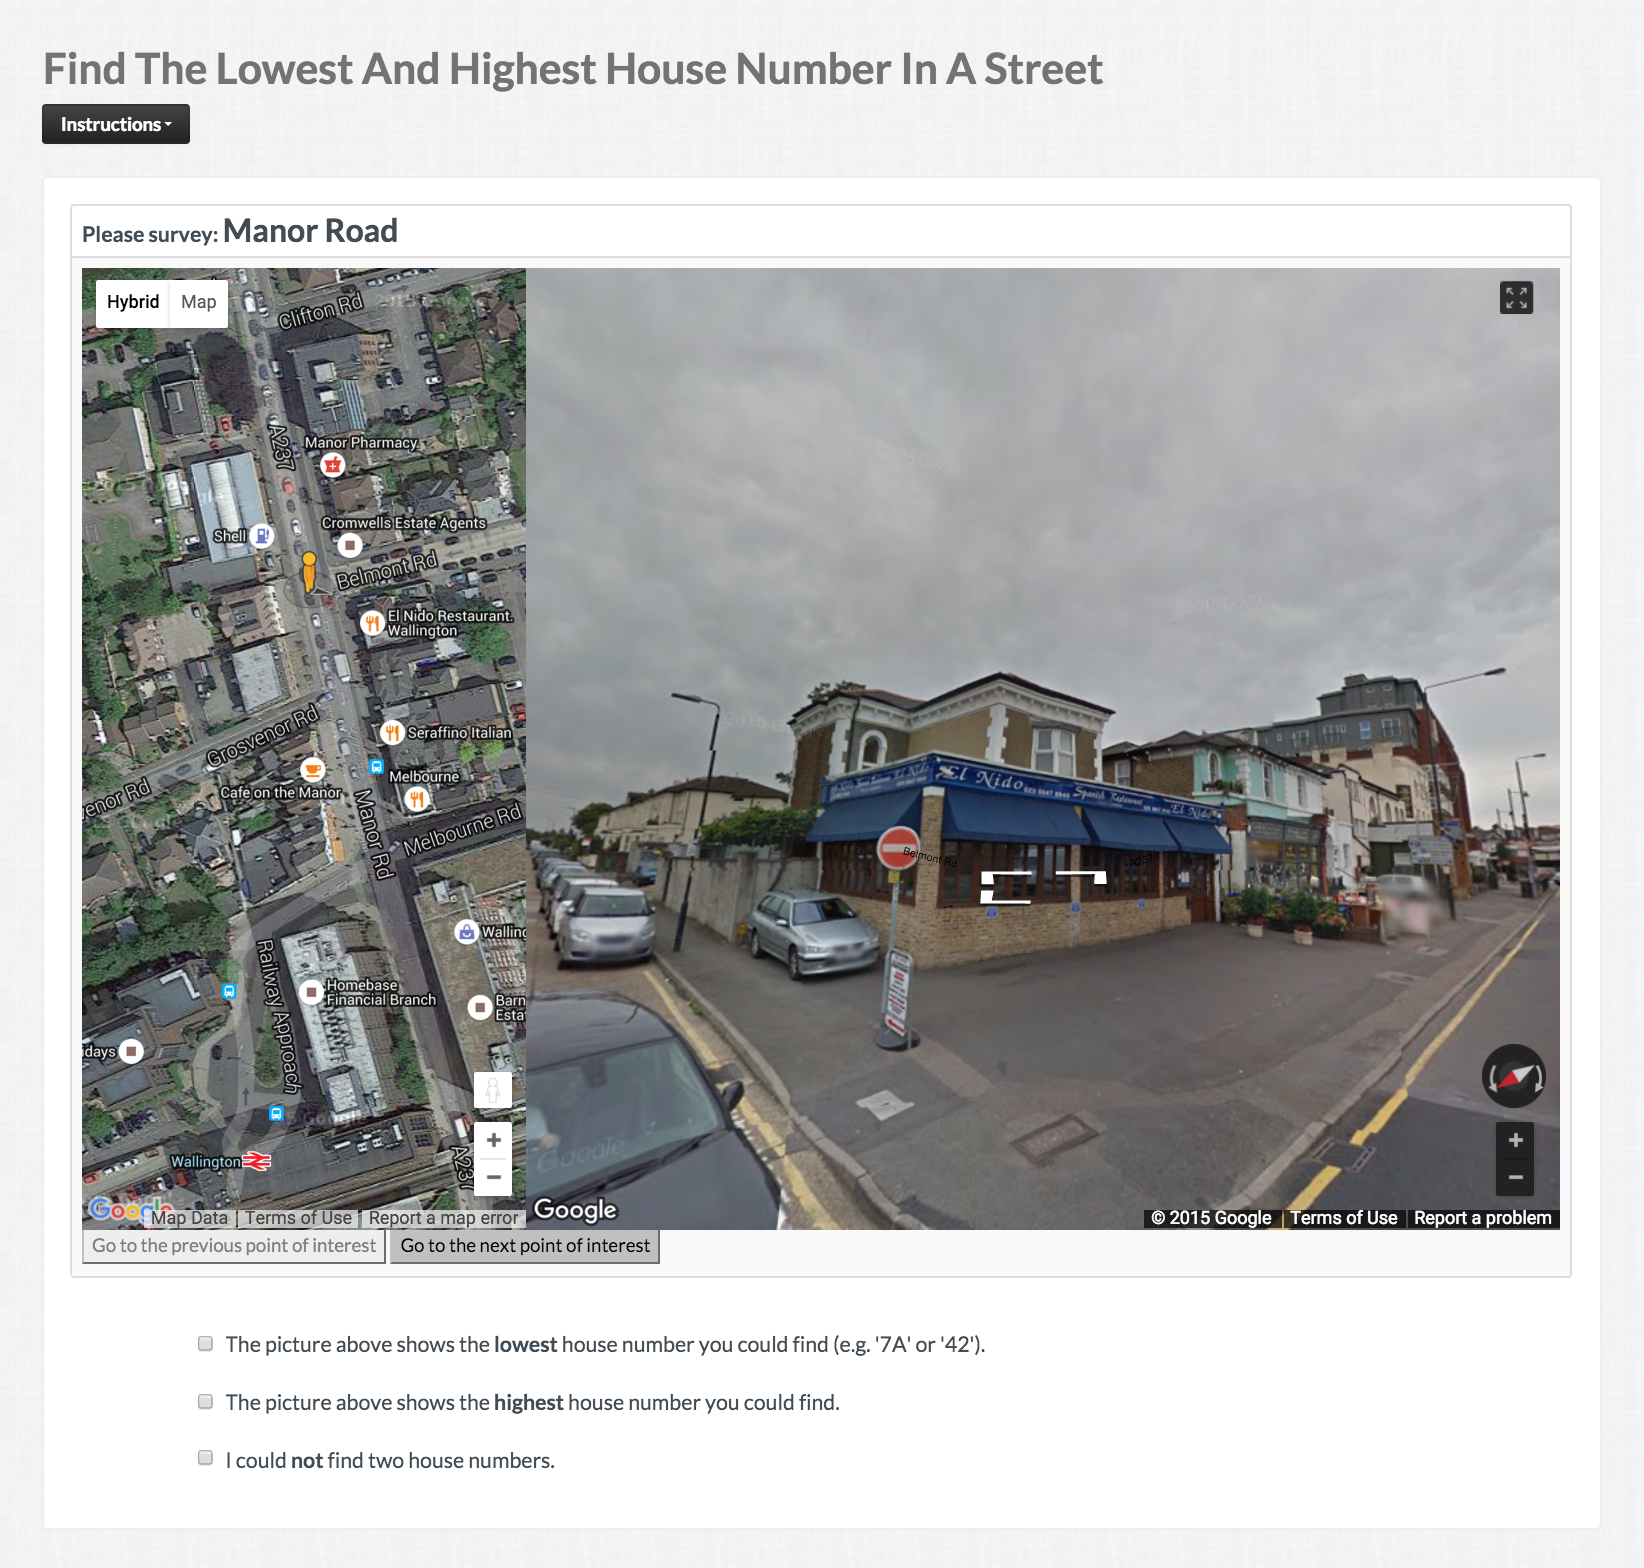
\includegraphics[width=0.95\textwidth]{virtual-survey-tool-01.png}
        	\caption{This picture should not be here, but apparently it is a nightmare in LaTeX.}
        	\label{fig:some_figure}
        \end{figure*}
        
        \paragraph{}

        The full code is available on GitHub at \url{https://github.com/Digital-Contraptions-Imaginarium/OLAF-yr2_lab/}.

    \subsubsection{Legal aspects}

    The choices made to get to the above approach may have legal implications that need to be taken into account, if it was decided to deploy the same methodology in the wild and - in particular - if the data that is the result of the process was published under an open licence, as originally intended. 
    
    To avoid any legal implications of this work, for the time being we are not publishing the data that was collected through our experiments, but just this paper and the source code that was used to build the system. [IS THIS IN CONTRADDICTION WITH THE CHOICE OF CROWDFLOWER'S DATA FOR EVERYONE? MOREOVER, THEIR SYSTEMS ARE NOT IN EUROPE]
    
    What is described below is our early understanding of three of the most interesting legal matters, that would need to be dealt with in future work. 

    \textbf{Personal data and privacy implications.} According to EU Data Protection Directive (95/46/EC\footnote{See \url{http://eur-lex.europa.eu/LexUriServ/LexUriServ.do?uri=CELEX:31995L0046:en:HTML}.} addresses are to be considered "personal data" even when they are not associated to information about who lives at those addresses, as they are "information relating to an identified or {\it identifiable} natural person" (no italics in the original). The directive describes a framework of good practices for member states to make into law that we would need to comply with.
    	
    \textbf{Annotation as derivative work.} Google Maps' terms of service \footnote{See \url{https://www.google.com/intl/en-GB_US/help/terms_maps.html}.} specify a restriction on producing "derivative works of the Content or any part thereof". We believe that asking crowdworkers to examine the Street View pictures and annotate them with the house numbers does not consist in deriving data as it would instead, for example, using a computer vision algorithm to systematically scan the data of pictures, or re-publishing any of machine-readable data that can be retrieved simply by calling Google's APIs. 
    
    \textbf{Database of places.} Again from Google's terms of service comes a restriction on using the services to create "a database of places or other local listings information". We believe that the terms allude to the possibility of re-using Google's data to create a competitor product to any of their services, which is not our case. In general, we also consider addresses as "attributes of places" (e.g. 10 Downing Street, London) rather than "places" (e.g. the UK Prime Minister official residence and office, at 10 Downing Street, London).
    	
    \subsubsection{Scalability}
    
        [THE CALL FOR PAPER EXPLICITLY SAYS THAT "EVIDENCE OF USE IN PRACTICE AND/OR DEMONSTRATION OF SCALABILITY IS REGARDED AS A PLUS"]
    
    \subsubsection{{[}description of additional conditions to test X{]}}
    \subsubsection{{[}description of additional conditions to test Y{]}}

[FIND SOME PLACE TO SAY WHY WE DON'T USE OPENSTREETMAP, BECAUSE SOMEONE WILL ASK. THE ANSWER IS THAT ITS LICENSING IS CONTROVERSIAL ACCORDING TO SOME: E.G. READ \cite{CentreforSpatialLawandPolicy:2014tx}]
    


\section{Experiment design}

\subsection{Research hypothesis}

Our work was centred around the hypothesis below:

\begin{enumerate}

    \item Paid crowdsourcing can be used to address some of the limitations of VGI, e.g. to survey streets on demand, quickly and reliably without the need to wait for a volunteer to offer herself for the task.
    
    \item Paid crowdsourcing can be effective at image labelling tasks that are more complex than what is commonly found in literature, as in the case of finding house numbers - or the lack thereof - in interactive visualisations of streets as in Google Street View.

    \item Effective workflow systems can be implemented by using just the native functionality of third party crowdsourcing services in the cloud such as CrowdFlower, hence maximising the system scalability and availability in respect to deploying custom components (code, application and database servers etc.)

    \item An iterative crowdsourcing workflow is more performing...
    
\end{enumerate}

To test these hypothesis, we carried out two experiments. Workers were offered to browse a street through a combination of Google Maps and Google Street View and asked to identify the lowest and the highest house numbers. The systems implementing the experiments were fully hosted on CrowdFlower, and only Google and CrowdFlower's native functionality was used, complemented by some "offline" scripting aimed at pre-processing the dataset and consolidating the results.

To test the first and second hypothesis, the potential for the community of Workers to converge on consensus on some of the streets was assessed, targeting a high degree of statistical confidence on the results.

To test the fourth hypothesis, two different approaches to judgement collection were implemented and their performance compared, both aiming at achieving results of equivalent quality.

The systems of the two experiments were indistinguishable from a Worker point of view. Participants used the same user interface, were paid the same amount etc.

\subsection{Dataset}

\subsection{Evaluation metrics}

We evaluate the performance of the approach as the average total cost per road required to reach Worker consensus. The lower the cost, the more effective the approach.

\subsection{Experimental conditions}

\textbf{Experiment 1} {\it Judgement collection: iterative, 5 judgements per road. Source dataset: the full sample of 184 roads, in "rounds" of max 10 roads depending on availability, chosen according to prioritisation. As road reach consensus, they are removed from the following round to make room for more roads. Stop condition: either (i) a total 400 judgements is collected or, (ii) consensus is reached on all roads, or (iii) at completion of any iteration, the number of total duplicate judgements by reliable Workers is higher than the number of unique judgement, whichever condition is verified first. Consensus: Fleiss kappa of 0.6 on roads where house numbers could be found, 0.8 on roads where house numbers could not be found, calculated at completion of each iteration.} 

\textbf{Experiment 2} {\it Judgement collection: one-shot, with a minimum of **** judgements and a maximum of **** per road. Collection is stopped on a road by road basis when consensus is reached. Source dataset: the same set roads that were subject to judgement in any round of Experiment 1. Stop condition: either (i) the same total number of judgements of Experiment 1 is collected, or (ii) consensus is reached on all roads, whichever condition is verified first. Consensus: simple agreement \% of Workers equivalent or superior to the worst case scenario Fleiss kappa of Experiment 1, calculated at completion of each judgement\footnote{CrowdFlower provides natively the functionality to continue judgement collection on each road until a target simple agreement x\% between Workers is achieved. Differently than Fleiss' kappa that was used in experiment 1, this does not take into consideration the distribution of judgements in disagreement. It is possible, though, to calculate a simple agreement \% that is statistically equivalent or better, for each combination of number of judgements and target kappa. E.g. the smallest simple agreement \% that can achieve a Fleiss' kappa of 0.8 on 30 judgements is 90\%, that is like saying that 27 Workers were in agreement, whatever the judgements were by the other workers.}.} 

\section{Results}

The result of the experiment is summarised in tables \ref{table:distribution-of-workers} and \ref{table:judgements-summary} below. 

After three consecutive iterations and a total of 150 judgements per road by 80 Workers, the number of total duplicate judgements by reliable Workers was higher than the number of unique judgements, hence triggering the stop condition. 

18.75\% of Workers failed the simple test of copying the name of the road in the form, and were not considered trustworthy. 

Agreement could be reached on four streets only at the end of those three rounds. All roads were identified as not having house numbers.

Collection was reprised at a later point in time to attempt leveraging a different Worker base, through three additional rounds. The judgements of 41 additional Workers were collected, achieving consensus on three more roads. 

\begin{table}[]
\centering
\begin{tabular}{|l|c|c|l|l|}
\hline
                   & \multicolumn{1}{l|}{\begin{tabular}[c]{@{}l@{}}Tot. no. of \\ Workers\end{tabular}} & \multicolumn{1}{l|}{\begin{tabular}[c]{@{}l@{}}No. of new \\ Workers\end{tabular}} & \begin{tabular}[c]{@{}l@{}}No. of \\ reliable\\ Workers\end{tabular} & \begin{tabular}[c]{@{}l@{}}\% of \\ reliable \\ Workers\end{tabular} \\ \hline
First three rounds & 80                                                                                  & -                                                                                  & 65                                                                   & 81.25\%                                                              \\ \hline
All six rounds     & 121                                                                                 & 41                                                                                 & 97                                                                   & 80.16\%                                                              \\ \hline
\end{tabular}
\caption{Distribution of Workers across rounds}
\label{table:distribution-of-workers}
\end{table}



\begin{table}[]
\centering
\begin{tabular}{|l|l|l|l|}
\hline
                   & \begin{tabular}[c]{@{}l@{}}No. of \\ reliable\\ Workers\end{tabular} & \begin{tabular}[c]{@{}l@{}}No. of non-duplicate\\ judgements\end{tabular} & \begin{tabular}[c]{@{}l@{}}No. of roads\\ where consensus\\ was achieved\end{tabular} \\ \hline
First three rounds & 65                                                                   & 117                                                                       & 4                                                                                     \\ \hline
All six rounds     & 97                                                                   & 227                                                                       & 7                                                                                     \\ \hline
\end{tabular}
\caption{Judgement numbers and consensus summary}
\label{table:judgements-summary}
\end{table}

The graph below illustrates how Fleiss kappa variated...



% \section{Literature review}
\section{Discussion and conclusion}

[NOTE ABOUT THE OPPORTUNITY TO MANAGE HOW THE RESULTS NATURALLY CLUSTER AROUND A FEW HIGHEST HOUSE NUMBERS, AS WORKERS MAY MISS SOME PARTS OF THE ROAD, THIS SHOULD BE DISCUSSED IF IT HAPPENS OFTEN, AFTER OBSERVING LARGER VOLUMES OF SUBMISSIONS]

\textbf{Acknowledgements.} [WRITE THIS, NOTHING REVEALING IF THE REVIEW IS BLIND]

\documentclass{article}
\usepackage{url}
\begin{document}
\nocite{*}
\bibliography{main}
\bibliographystyle{splncs03}
\end{document}


\end{document}

